\section{Debugging Tools}

\subsection{GDB (GNU Debugger)}
GDB adalah standar industri untuk penelusuran \textit{runtime} kesalahan logika. Sangat berguna untuk melihat jejak tumpukan (\textit{backtrace}) saat kompilator mengalami \textit{segmentation fault}.

\subsection{Sanitizers: Pembersihan Otomatis}
Bagi pengembang kompilator modern, menggunakan \compiler{Sanitizers} (seperti ASan dan MSan) seringkali lebih efisien daripada debugging manual \cite{jhu2024compilers}.
\begin{enumerate}
    \item \textbf{AddressSanitizer (ASan)}: Mendeteksi penggunaan memori setelah dibebaskan (\textit{use-after-free}) dan luapan buffer (\textit{buffer overflow}) secara otomatis dengan \textit{slowdown} minimal.
    \item \textbf{MemorySanitizer (MSan)}: Mendeteksi pembacaan nilai dari memori yang belum diinisialisasi.
    \item \textbf{ThreadSanitizer (TSan)}: Membantu mendeteksi \textit{race conditions} jika kompilator mendukung pemindaian paralel.
\end{enumerate}

\subsection{Valgrind}
Meskipun lebih lambat dari ASan, Valgrind tetap menjadi alat utama untuk deteksi kebocoran memori (\textit{memory leaks}) karena tidak memerlukan kompilasi ulang kode sumber.

\begin{figure}[!htbp]
    \centering
    \adjustbox{max width=0.8\textwidth,center}{%
    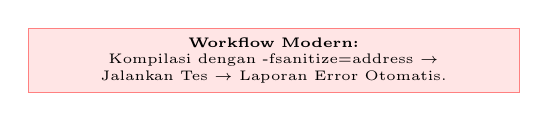
\begin{tikzpicture}[
        node/.style={rectangle, draw=red!50, fill=red!10, text width=6cm, font=\tiny, align=center}
    ]
    \node[node] (asan) {
        \textbf{Workflow Modern:}\\
        Kompilasi dengan \code{-fsanitize=address} $\rightarrow$ Jalankan Tes $\rightarrow$ Laporan Error Otomatis.
    };
    \end{tikzpicture}%
    }
    \caption{Debugging Cepat menggunakan Sanitizers}
\end{figure}
